\documentclass[
  25pt,         % default font size: 17pt, 20pt(default), 25pt, 30pt
  a4paper,
  landscape,
  Screen4to3,
% headrule,
  footrule ]{foils}

\usepackage[%
    a4paper,%
    bookmarks=false,%
    colorlinks=false,%
    pdftitle={404050 VU/3 VU Empirical Economics: Impact Evaluation, Fall 2023},%
    pdfauthor={Andreas Steinmayr}%
    ]{hyperref}

\usepackage[OT1]{fontenc}
\usepackage[latin1]{inputenc}
\usepackage{hyperref}
\usepackage{color}
\usepackage{xcolor}
\usepackage{verbatim}
\usepackage{amsmath}
\usepackage{amssymb}
\usepackage{bm}
\usepackage{graphicx}
\usepackage{ifthen}
\usepackage{hyperref}
\usepackage{tikz}

\input{jo-math}

\newcommand{\Perp}{\perp \! \! \! \perp}

%================================================================
% Global macros
%================================================================
 \MyLogo{Andreas Steinmayr, 404050 VU/3 VU Empirical Economics: Impact Evaluation, Fall 2023}
 \rightfooter{\thepage}

 \newcommand{\sectiontitle}{}

%================================================================
% Toggle lecture / print version
%================================================================

\newboolean{lecture}

\setboolean{lecture}{true}

\ifthenelse{\boolean{lecture}}{%
  \usepackage[
      display,        % enable dynamic features for presentations
      whitebackground % enable blue-on-white colors for presentations
  ]{texpower}
  \newcommand{\textclr}{\usecolorset{whitebackground}}
  \newcommand{\lecture}[1]{#1}
  \newcommand{\lecturep}[1]{#1}
  }
  {
  \usepackage{texpower}
  \newcommand{\textclr}{\color{black}}
  \renewcommand{\pause}{}
  \newcommand{\lecture}[1]{}
  \newcommand{\lecturep}[1]{\phantom{#1}}
  }

\newcommand{\wait}{\pause \vspace{-1mm}}

\newcommand{\xx}{\item[{\small $\bullet$}]}

\newcommand{\definition}{{\bf Definition:}\;}
\newcommand{\result}{{\bf Result:}\;}
\newcommand{\namedresult}[1]{{\bf Result~(#1):}\;}

 \addtolength{\textheight}{\headheight +\headsep +\footskip +.3in}
 \setlength{\headheight}{0pt} \setlength{\headsep}{0pt}
 \setlength{\footskip}{0pt} \setlength{\foilheadskip}{-.2in}


%================================================================
% Colors
%================================================================

\definecolor{red}{rgb}{1,0,0}
\definecolor{green}{rgb}{0,1,0}

\boxedsteps % turn on boxedsteps


%================================================================
\begin{document}

\setlength{\parindent}{0pt}




%================================================================
\foilhead{VU Empirical Economics: Impact Evaluation}

\thispagestyle{empty}

\begin{center}

\textbf{Causal inference and counterfactuals} \\  \bigskip  \bigskip \bigskip
 \bigskip \bigskip \bigskip


Andreas Steinmayr \\ 
 \bigskip \bigskip \bigskip

University of Innsbruck \bigskip


Fall 2023 \\ \bigskip  \bigskip \bigskip \bigskip


\end{center}

\small{\textit{Core reading: Gertler, chapters 3; Cunningham, chapters 3 and 4}}


%================================================================
\foilhead{Causal inference}
\begin{small}
\textit{Remember:} Impact evaluations seek to answer cause-and-effect questions precisely.


The \textbf{causal impact} of a program on an outcome is the difference between
\bi
\xx the outcome with the program
\xx and the same outcome without the program
\ei
To put it another way, we would like to measure the outcome \textbf{at the same point in time for the same unit}, but in \textbf{two different states of the world}.

Obtaining these measures is impossible because we only observe one state of the world. We need a framework to think about the problem.
\end{small}


%================================================================
\foilhead{RCM: Observed and potential outcomes}

\bi

\x In \textit{traditional} econometrics, we use \textbf{observed outcomes $Y$} 

\vsm

\x The literature on program evaluation builds on the notion that
each member of the population can be characterized by (two)
\textbf{potential outcomes}: \vsm
    \bea
    Y^0 & : & \mbox{potential outcome if not treated} \nonumber
    \\[-2mm]
    Y^1 & : & \mbox{potential outcome if treated} \nonumber
    \eea

\vsm \vsm
\x Causality is based on \textbf{comparison of potential outcomes}
\vsm
\bi 
\xx Requires counterfactual thinking
\ei
\x Statistical framework: \textit{Rubin Causal Model} (Rubin 1974)
\ei


%================================================================
\foilhead{RCM: Observed and potential outcomes}

\bi

\x The treatment indicator is defined as
    \bdm
    W = \left\{
    \begin{array}{r@{\quad}l}
    0 & \mbox{if not treated}  \\
    1 & \mbox{if treated}
    \end{array} \right.
    \edm

\vsm \vsm

\x We will stick to binary treatments for most of the course but at times also consider situations in which the treatment variable can take different values (``treatment intensities'').

\x After treatment is applied, only one of the potential outcomes is realized:
    \bdm
    Y=Y^W= \left\{
    \begin{array}{r@{\quad}l}
   Y^0 & \mbox{if W=0}  \\
    Y^1 & \mbox{if W=1}
    \end{array} \right.
    \edm

\vsm \vsm

\ei

%================================================================
\foilhead{Stable Unit Treatment Value Assumption (SUTVA)}

\bi

\x Treatment of some unit (\eg, a person) only
affects that persons outcome -- this is often referred to as
SUTVA.

\x No multiple versions of the program (no good/bad pills)
\x Rules out general equilibrium effects - program evaluation usually is about partial equilibrium analysis. 
\bi 
\xx For example, the fact a some training raises one person's skill level
might imply that another person looses her job if the number of
jobs is fixed.
\ei
\ei

%================================================================
\foilhead{The perfect clone}

\begin{center}
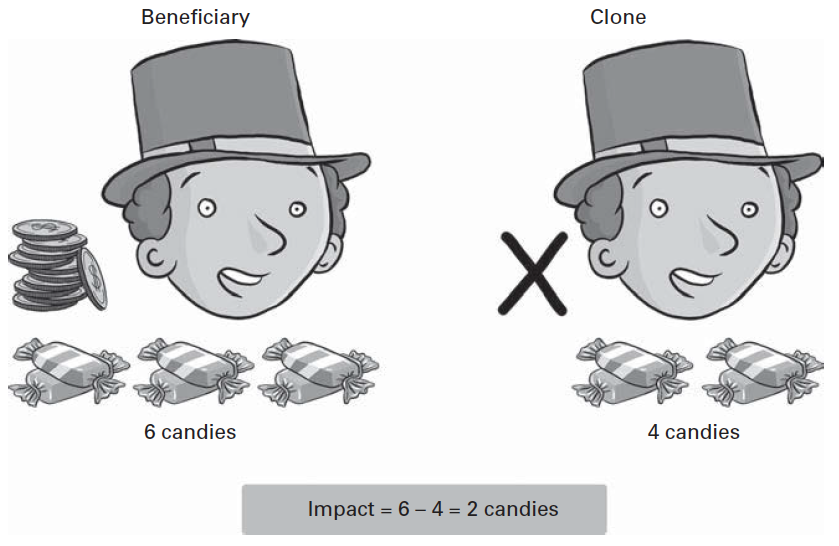
\includegraphics[width=0.8\textwidth]{figures/perfect_clone}
\end{center}

%================================================================
\foilhead{RCM: Causal effect}

\bi

\x The \textbf{treatment effect} is the difference of the two
hypothetical outcomes: \vsm
    \bdm
    Y^1 - Y^0
    \edm

\vsm

\x While we can think hypothetically about this quantity, \textbf{we can't
observe it for any specific member of the population}.
\vsm
\x This is the fundamental evaluation problem 
\vsm
\x The unobserved outcome is what we call the \textit{Missing Counterfactual}
\vsm
\x The evaluation problem is a missing data problem

\ei

%================================================================
\foilhead{Manipulation}

Causal questions require careful description of manipulation to be well defined:

"She did not get this job because she is a woman."

What is the manipulation?
\vsm
\bi 
\x Change chromosome after conception
\vsm
\x Change gender on written job application
\ei

Very different manipulations, and probably different causal effects!

Discussion: If we cannot think of a manipulation, why are we interested in the effect?

%================================================================
\foilhead{RCM: Average Treatment Effect}

\bi

\x Instead of individual treatment effects, we can focus on the average effect of the
treatment.
\x We call this the \textbf{average treatment effect} (ATE)
\vsm
    \bdm
    \tau_{ATE} = \E[Y^1 - Y^0] \, ,
    \edm

\vsm \vsm

\x Note that we make no assumption that the effect is the same for everyone.
 \vsm
\x We have to think about for which group we are identifying the ATE. 

\ei


%================================================================
\foilhead{RCM: Average Treatment Effect}

\bi

\x The average treatment effect, $\tau_{ATE}$ is an unknown
population parameter. Thus, we assign a Greek letter to it, as in
the case of a population mean where we define $\E(y)=\mu$. The
evaluation literature prefers using acronyms (as in: ``We estimate
the ATE.'')

\vsm

\x There is a crucial difference between the population mean,
$\E(y)$, and the average treatment effect, $\E[Y^1-Y^0]$:
    \bi
    \xx With a random sample from the population, $\mu$ can be estimated
    by the sample analog of $\E(y)$: $\widehat{\mu} = \frac{1}{N} \sum_{i=1}^N y_i = \bar{y}$.
    \vs
    \xx $\tau_{ATE}$ cannot be estimated by a sample average without
    additional assumptions. (Why?)
    \ei

\ei


%================================================================
\foilhead{RCM: Average Treatment Effect on the Treated}

\bi

\x Another population quantity of interest is the \textbf{average
treatment effect on the treated} (ATT):
    \vsm
    \bdm
    \tau_{ATT} = \E(Y^1 - Y^0|W=1) \, ,
    \edm

\vsm \vsm

which is the expected effect of treatment on the outcome for a
randomly drawn member of the sub-population that received the
treatment.

\vsm

\x The ATT can't be estimated by a sample
average without additional assumptions either.

\ei

%================================================================
\foilhead{RCM: Average Treatment Effect on the Non-treated}

\bi

\x Another population quantity of interest is the \textbf{average
treatment effect on the non-treated} (ATNT):
    \vsm
    \bdm
    \tau_{ATNT} = \E[Y^1 - Y^0|W=0] \, ,
    \edm

\vsm \vsm

which is the expected effect of treatment on the outcome for a
randomly drawn member of the sub-population that did not receive the
treatment.

\ei

%================================================================
\foilhead{Exercise}


Use the following dataset to estimate the ATE, ATT, and ATNT. Note: Quantities in italics are not observed in real world data but you can use them here.
\begin{center}
\begin{small}
\begin{tabular}{ccccc}\hline 
$i$&$W_i$&$Y_i^0$&$Y_i^1$&$\Delta_i=Y_i^1-Y_i^0$\\\hline 
 1  & 0 & 6 & \textit{8} &  \\
2   & 0 & 6 & \textit{9} &  \\
3  & 0 & 9 & \textit{11} &  \\
4  & 1 & \textit{8} & 12 &  \\
 5  & 1 & \textit{7} & 10 &  \\
 6  & 1 & \textit{2} & 6 &  \\
 7   & 1 & \textit{10} & 13 &  \\
 8   & 1 & \textit{5} & 9 &  \\
 9   & 0 & 7 & \textit{10} &  \\
10   & 0 & 10 & \textit{12}&  \\\hline                      
  \end{tabular}
\end{small}
\end{center}

%ATNT: 2.4, ATT: 3.6, ATE: 3


%================================================================
\foilhead{No information bounds}

\bi 
\x What can we say about causal parameters without data and assumption?
\x Even without assumptions and data, we know that the treatment effects are in some interval if the expectations of the outcome variable of interest are bounded
\x Assumption BS: Bounded support of potential outcomes: $\E[Y^0|W=1]\in[\underline{Y},\overline{Y}]$ and $\E[Y^1|W=0]\in[\underline{Y},\overline{Y}]$
\ei
%================================================================
\foilhead{No information bounds: example}
\bi 

\x Example: ATT of college degree on labor supply. Labor supply is a binary variable and thus bounded. 
\pause
\x Without any data we can say
    \vsm
    \bea
    \tau_{ATT} = \E[Y^1|W=1] - \E[Y^0|W=1] \nonumber
    \eea
\x Upper bound of effect: $\overline{\tau_{ATT}} = \overline{Y} - \underline{Y}$
\x Lower bound of effect:   $\underline{\tau_{ATT}} = \underline{Y} - \overline{Y}$
\x Length of bounds is $2*(\overline{Y}-\underline{Y})$
\ei

\foilhead{No information bounds: example}


With observable data containing $Y$ and $W$ the bounds for the ATT shrink to:
\pause
\bi 
\x Upper bound of effect: $\overline{\tau_{ATT}} =\E[Y|W=1] - \underline{Y}$
\x Lower bound of effect:   $\underline{\tau_{ATT}} = \E[Y|W=1]- \overline{Y}$
\x Length of bounds is $(\overline{Y}-\underline{Y})$
\ei
\pause
Data reduce uncertainty (interval) by 50\%

\vsm
Assumptions have to reduce the other 50\%




%================================================================
\foilhead{The na\"{i}ve estimator}

\bi

\x The estimation problem for both $\tau_{ATE}$ and $\tau_{ATT}$
results from the fact that we never observe both $Y^0$ and $Y^1$
at the same time.

\vsm

\x We only observe realized outcomes and the treatment
indicator: \vsm \vsm
    \bea
    y &=& (1-w) \, y_0 + w \, y_1 \nonumber \\
      &=& y_0 + w(y_1-y_0) \nonumber
    \eea

\vsm \vsm \vsm

\x With a sample of $(Y,W)$, why can't we take the simple difference  \vsm  
    \bdm
    \hat{\tau}_N = \bar{y}_{w=1} - \bar{y}_{w=0}
    \edm
 \vsm \vsm \vsm

\x which would correspond to the following regression: 
 \vsm
        \bdm
    y = \beta_0 + \beta_1 w + u
    \edm
 \vsm \vsm \vsm \vsm
\ei

%================================================================
\foilhead{Example: Roy model}

Suppose there are only two occupations in the world: economists and accountants. Suppose non-wage aspects of the jobs are the same. 

Earnings of accountants are given by:
    \vsm
    \bdm
    Y^0 \sim N(60000,5000) 
    \edm
\vsm   \vsm    \vsm    \vsm 
    
Earnings of economists are:
    \vsm
    \bdm
    Y^1 \sim N(60000,10000) 
    \edm
\vsm   \vsm    \vsm    \vsm 

In addition, we assume the correlation between accounting and economist wages is high: 0.84. If you're going to be a good economist, it's very likely you'll also be good at accounting.

%================================================================
\foilhead{Example: Roy model}
\begin{small}


Now let's build a model of occupation selection. Because non-wage aspects of both jobs are the same, the worker picks the one that pays the most. Her observed earnings are

    \vsm
    \bdm
    y_i = max(y^0_i,y^1_i)
   \edm
\vsm   \vsm   

Note that here $Y_i$ is written in lower case because it is the realization of a random variable. Because both $Y^0_i$ and $Y^1_i$ are lower-case on the right-hand side of the equation, we are assuming that our agent knows what her earnings would be in each occupation before she decides to be an economist or accountant. Let $W_i = 1$ indicate she chooses economics.
Now, since we are devising the model, we can do something we can't do in real life: observe the potential earnings of the entire population.
\end{small}

%================================================================
\foilhead{Example: Roy model}

\begin{center}
\begin{small}
\begin{tabular}{lccc}\hline 
 & Accountants & Economists & Total \\
Accounting earnings & 58,346 & \textit{61,648} &  \textit{59,996}  \\
Economics earnings &  \textit{54,469} & 65,519 & \textit{59,991} \\ \hline
N & 500,245 & 499,755 & 1,000,000 \\ \hline            
  \end{tabular}
\end{small}
\end{center}

Quantities in italics are the unobserved counterfactuals and not observed in real world data.

We, as economists, want to know what impact choosing to be an economist has on economists' earnings relative to the counterfactual of them being accountants. We have defined treatment as being an economist, so what treatment parameters are we interested in?

%================================================================
\foilhead{Example: Roy model}
\begin{small}
The na\"{i}ve estimator gives us 
\vsm
    \bea
    \hat{\tau}_N &=& \bar{y}_{w=1} - \bar{y}_{w=0} = \bar{y}^1_{w=1} - \bar{y}^0_{w=0} \nonumber \\
    &=&65,519-58,346=7,173 \nonumber
    \eea
\vsm

This is na\"{i}ve as it assumes that a good estimate of economists' counterfactual accounting earnings is the observed accountants' accounting earnings.

Since we got to observe all potential outcomes in this exercise, we can calculate what the real gain from becoming economists is for the people who become economists.
\vsm
    \bea
    \hat{\tau}_{ATT} &=& \bar{y}^1_{w=1} - \bar{y}^0_{w=1} =65,519-61,648=3,871 \nonumber
    \eea
\end{small}

%================================================================
\foilhead{Example: Roy model}

Alternatively, you could have estimated the impact of becoming economists for those who actually became accountants

\vsm
    \bea
    \hat{\tau}_{ATNT} &=& \bar{y}^1_{w=0} - \bar{y}^0_{w=0} =54,469-58,346=-3,877 \nonumber
    \eea


It looks like those who became accountants made the right choice: they would have been worse off if they had become economists! This again shows why the na\"{i}ve estimator is so bad.

%================================================================
\foilhead{Example: Roy model}

Finally, you may want to know what the impact would be if we made everyone become economists.
\vsm
    \bea
    \hat{\tau}_{ATE} &=& \bar{y}^1 - \bar{y}^0 =59,991-59,996=-5 \nonumber
    \eea

All three of these parameters are meaningful, and our na\"{i}ve estimator gives
us none of them.


%================================================================
\foilhead{The selection problem}

\bi
\x This na\"{i}ve estimator implicitly assumes that
    \bea
    \E[Y|W=1] &=& \E[Y^1|W=1] \; = \; \E[Y^1] \nonumber \\
    \E[Y|W=0] &=& \E[Y^0|W=0] \; = \; \E[Y^0] \nonumber
    \eea
\x In traditional econometrics, we called this \textit{ceteris paribus}
\x We call violations of these assumptions the \textbf{Selection Problem}
\ei

%================================================================
\foilhead{Exercise}

\bi
\x Use the na\"{i}ve estimator for the small dataset.
\x Study the potential outcomes. Is the assumption behind the na\"{i}ve estimator fulfilled? 
\ei

%================================================================
\foilhead{The selection problem: a valid comparison group}

\begin{center}
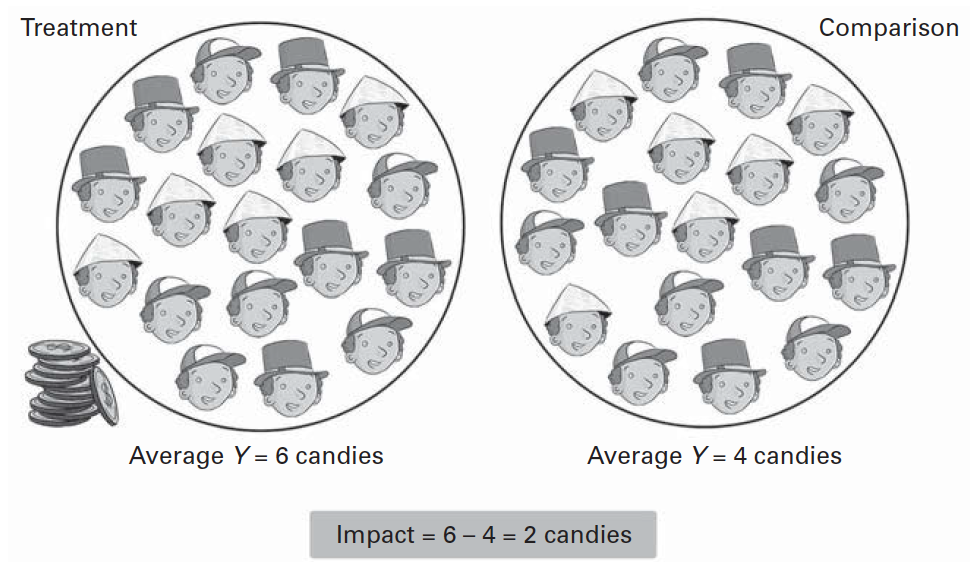
\includegraphics[width=0.8\textwidth]{figures/valid_comparison}
\end{center}

%================================================================
\foilhead{The selection problem}

\bi 
\x Dealing with the selection problem is often the biggest challenge in policy evaluation
\vsm
\x The selection problem arises because we only observe certain/selected people in the treated state
\vsm
\bi 
\xx Participants are a nonrandom sample from the eligible population
\xx They are different from those not treated
\xx They are also different from themselves prior to the start of the treatment
\ei
\vsm
\x {\textit{Different}} refers to: they have different potential outcomes
\vsm
\x \textbf{Why did these people get treated while others did not?}
\ei

%================================================================
\foilhead{Two types of selection}

\bi 
\x {\textbf{Selection on Observables}}
\vsm
\bi 
\xx Participants are different from non-participants in terms of observable characteristics, i.e. characteristics for which we have measures in our data.
\ei
\x {\textbf{Selection on Unobservables}}
\vsm
\bi 
\xx Participants are different from non-participants in terms of unobservable characteristics.
\ei
\vsm
\x The type of selection has important implications for the empirical methods we can use.
\vsm
\x How did we think about selection in our \textit{standard} econometrics class?
\ei


%================================================================
\foilhead{No information bounds}

\bi 
\x What can we say about causal parameters without data and assumption?
\x Manski (1989, 1990) and Robins (1989) show that even without assumptions and data, we know that the treatment effects are in some interval if the expectations of the outcome variable of interest are bounded
\x Assumption BS: Bounded support of potential outcomes: $\E[Y^0|W=1]\in[\underline{Y},\overline{Y}]$ and $\E[Y^1|W=0]\in[\underline{Y},\overline{Y}]$
\ei
%================================================================
\foilhead{No information bounds: example}
\bi 

\x Example: ATT of college degree on labor supply. Labor supply is a binary variable and thus bounded. 
\x Without any data we can say
    \vsm
    \bea
    \tau_{ATT} = \E[Y^1|W=1] - \E[Y^0|W=1] \nonumber
    \eea
\x Upper bound of effect: $\overline{\tau_{ATT}} = \overline{Y} - \underline{Y}$
\x Lower bound of effect:   $\underline{\tau_{ATT}} = \underline{Y} - \overline{Y}$
\x Length of bounds is $2*(\overline{Y}-\underline{Y})$
\ei

\foilhead{No information bounds: example}
\bi 

\x With observable data containing $Y$ and $W$ the bounds for the ATT shrink to:
\bi 
\xx Upper bound of effect: $\overline{\tau_{ATT}} =\E[Y|W=1] - \underline{Y}$
\xx Lower bound of effect:   $\underline{\tau_{ATT}} = \E[Y|W=1]- \overline{Y}$
\xx Length of bounds is $(\overline{Y}-\underline{Y})$
\ei
\pause
\x Data reduce uncertainty (interval) by 50\%
\vsm
\x Assumptions have to reduce the other 50\%
\ei

\foilhead{Literature}

\begin{footnotesize}
\bi 
\x Manski, C. F. (1989): The Anatomy of the Selection Problem, \textit{Journal of Human Resources}, 24, 343-360.

\x Manski, C. F. (1990): Nonparametric Bounds on Treatment Effects, \textit{American Economic Review, Papers and Proceedings}, 80, 319-323.

\x Robins, J. M. (1989): The Analysis of Randomized and Nonrandomized AIDS Treatment Trials Using a New Approach to Causal Inference in Longitudinal Studies", In: Sechrest, L., H. Freeman, A. Mulley (eds.), \textit{Health Service Research Methodology: A Focus on Aids}, 113-159, Washington, D.C.: Public Health Service, National Center for Health Services Research.

\x Roy, A. D. (1951): Some Thoughts on the Distribution of Earnings, \textit{Oxford Economics Papers}, 3(2), 135-146.

\x Rubin, D.B. (1974): Estimating Causal Effects of Treatments in Randomized and Non-randomized Studies, \textit{Journal of Educational Psychology}, 66, 688-701.
\ei
\end{footnotesize}


\end{document}
